\ifSTANDALONE
\section{Stepper Driver L6480} \label{sec:L6480}
\fi
\ifEMBED
\subsection{Stepper Driver L6480} \label{sec:L6480}
\fi

\ifEMBED
    % Dieses Kapitel ist eine Zusammenarbeit der Gruppen \BLDCTeams. 
    \BLDCcollab
\fi
    	Wie bereits im Kapitel \ref*{subsec:Ansteuerung} erwähnt, wird der L6480 von STMicroelectronics verwendet. 
	  	 \ifSTANDALONE
	  	 \subsection{Funktionsbeschreibung}
	  	 \fi
	  	 \ifEMBED
	  	 \subsubsection{Funktionsbeschreibung}
	  	 \fi
		 	Diese Schrittmotorensteuerung ist für den Betrieb von zweiphasigen (Vgl. Kpaitel \ref{wirkungsweise}) Schrittmotoren mit Mikrosteps (Vgl. Kapitel \ref{wirkungsweise}) geeignet. Der L6480 erreicht eine maximale Auflösung von einem 1/128 Schritt. Die Steuerung generiert intern die PWM- Signale für die Motorenansteuerung. Alternativ kann auch mit Einzelschritten oder Halbschritten gearbeitet werden. Die beiden H- Brücken werden extern mit N-Kanal MOSFETs realisiert. Es können Bewegungsprofile konfiguriert werden, so dass die Motoren definiert Anfahren, Abbremsen oder ein Punkt direkt angefahren werden kann. So kann der Aufwand bei der Mikrokontrollerprogrammierung verringert werden. Die Befehle werden über eine SPI- Schnittstelle übertragen. Die absolute Position ist in einem 22- Bit Register gespeichert. Der Bereich liegt dementsprechend zwischen \(-2^{21}\) und \(2^{21}-1\). \cite{Datasheet:L6480} 
		 \ifSTANDALONE
		 \subsection{Schnitstelle}
		 \fi
		 \ifEMBED
		 \subsubsection{Schnittstelle}
		 \fi
	  		Der steuernde Mikrocontroller benötigt 8 Pins für die Kommunikation mit dem L6480 \cite{Datasheet:L6480} : 
	  		\begin{longtable}{l l p{7cm}} \toprule
	  			\textbf{Pin} 	& \textbf{IO} 	& \textbf{Funktion} \\
	  			\midrule
	  			\endhead
	  			\multicolumn{3}{l}{\emph{Fortsetzung auf nächster Seite}} \\ \bottomrule \endfoot \endlastfoot 			
	  			\textbf{IO}\\ \addlinespace
	  			%\cmidrule{1-1}
	  			$\overline{FLAG}$& Output 				& Wird bei einem Fehler intern auf GND gezogen. \\ \addlinespace
	  			$\overline{BUSY}$ / SYNC & Output		& Wird während dem Ausführen eines Befehls intern auf GND gezogen.\\ \addlinespace
	  			$\overline{STBY / RESET}$& Input		& Standby- und Resetmodus, falls extern GND anliegt. \\ \addlinespace
	  			STCK			& Input			& Im Step-Clock- Mode führt jede positive Flanke an diesem Pin zu einem Schritt. \\ \addlinespace
	  			%\cmidrule{1-1}
	  			\textbf{SPI}\\ \addlinespace
	  			%\cmidrule{1-1}
	  			$\overline{CS}$	& Input			& Chip Select: Falls extern GND anliegt, startet die Kommunikation. Um die Kommunikation zu beenden, muss $\overline{CS}$ extern auf High gehalten werden. \\ \addlinespace
	  			CK				& Input			& Serial Clock: Synchronisierung der Kommunikation. \\ \addlinespace
	  			SDO				& Output		& Slave Data Out: Daten für den Mikrocontroller. \\ \addlinespace
	  			SDI				& Input			& Slave Data In: Befehle und Daten für den L6480. \\ \addlinespace
	  			\bottomrule
	  			\\
	  			\caption{Schnittstelle} 
	  			\label{Schnittstelle}
	  		\end{longtable}	
	  	\ifSTANDALONE	
	 	\subsection{Typical Application}
	 	\fi
	 	\ifEMBED
	 	\subsubsection{Typical Application}
	 	\fi
			 	\begin{figure}[h]
			 		\centering
			 		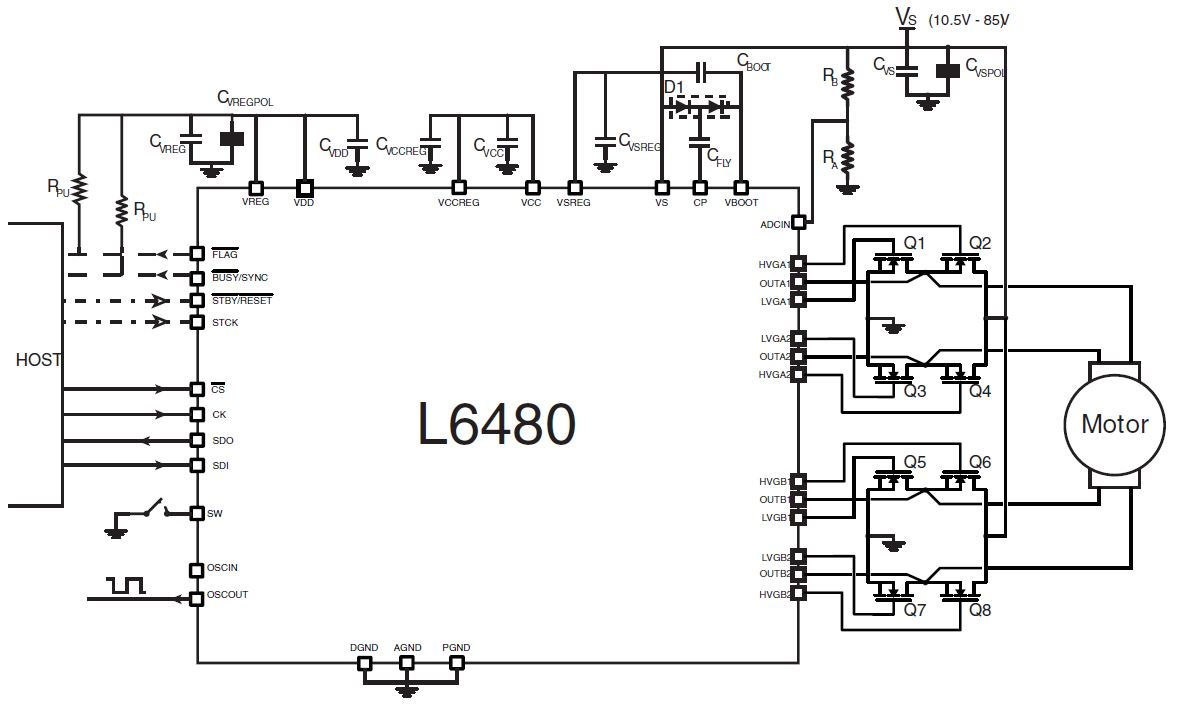
\includegraphics[width=12cm]{\EtPath/Bilder/typicalApp.jpg}
			 		\label{fig:typApp}
			 		\caption[Typical Application]{Typical Application \cite{Datasheet:L6480}}
			 	\end{figure}